 \documentclass[a4paper,10pt]{article}
\input{/Users/WannaGetHigh/workspace/latex/macros.tex}

\title{M3DA - TP 3: st\'er\'eovision dense}
\author{Fran\c cois \bsc{Lepan}}

\begin{document}
\maketitle

\section*{Introduction}

Dans le TP pr\'ec\'edent nous avons vu comment faire de la st\'er\'eovision via l'utilisation de "coins" et droites \'epipolaires . Cette m\'ethode permettait de faire de la reconstruction 3D bas\'e sur la g\'eom\'etrie des sc\`enes. Dans ce TP nous allons voir comment faire de la st\'er\'eovision avec non plus quelques pixels mais tous les pixels de l'image  ainsi que les niveaux de gris de la sc\`ene. \\

Afin de simplifier le probl\`eme on utilisera une configuration canonique. (\emph{cf.}~Fig.\ref{conf_canonique}). En effet dans cette configuration on va pouvoir directement calculer la disparit\'e qui est la diff\'erence entre les abscisses de deux points homologues. \\

La derni\`ere \'etape sera de calculer la disparit\'e en chaque point et la stocker dans une image nous donnant la carte des disparit\'es.

\begin{figure}[ht]
\begin{center}
	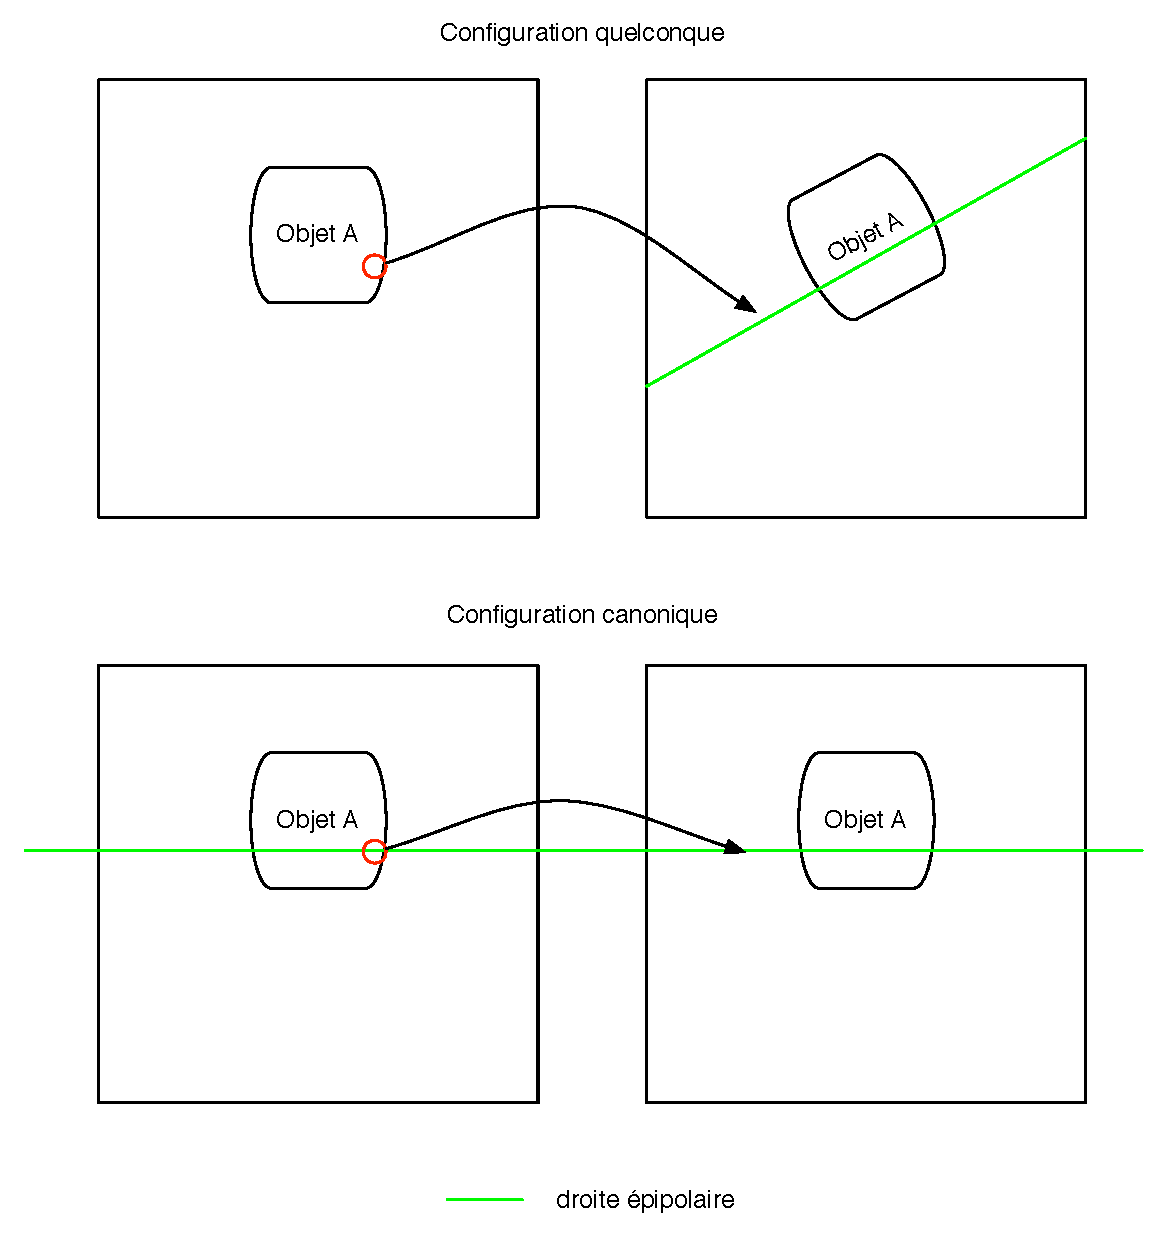
\includegraphics[width=7cm]{images/confi_canonique}
\end{center}
	\caption{En bas configuration canonique entre deux images d'une sc\`ene et en haut une configuration quelconque.}
	\label{conf_canonique}
\end{figure}

\section{Similarit\'e par SSD}

La premi\`ere \'etape est de maximiser la similarit\'e et donc minimiser la dissimilarit\'e entre deux voisinages. \\

Pour cela on va (\emph{cf.}~Fig.\ref{calcule_SSD}):
\begin{itemize} 
	\item d\'efinir un voisinage centr\'e sur chaque pixel,
	\item utiliser une fonction de dissimilarit\'e sur les deux voisinages courant,
	\item et enfin on va op\'erer un d\'ecalage sur l'une des images afin de rep\'erer des voisinages similaires.
\end{itemize}

\begin{figure}[ht]
\begin{center}
	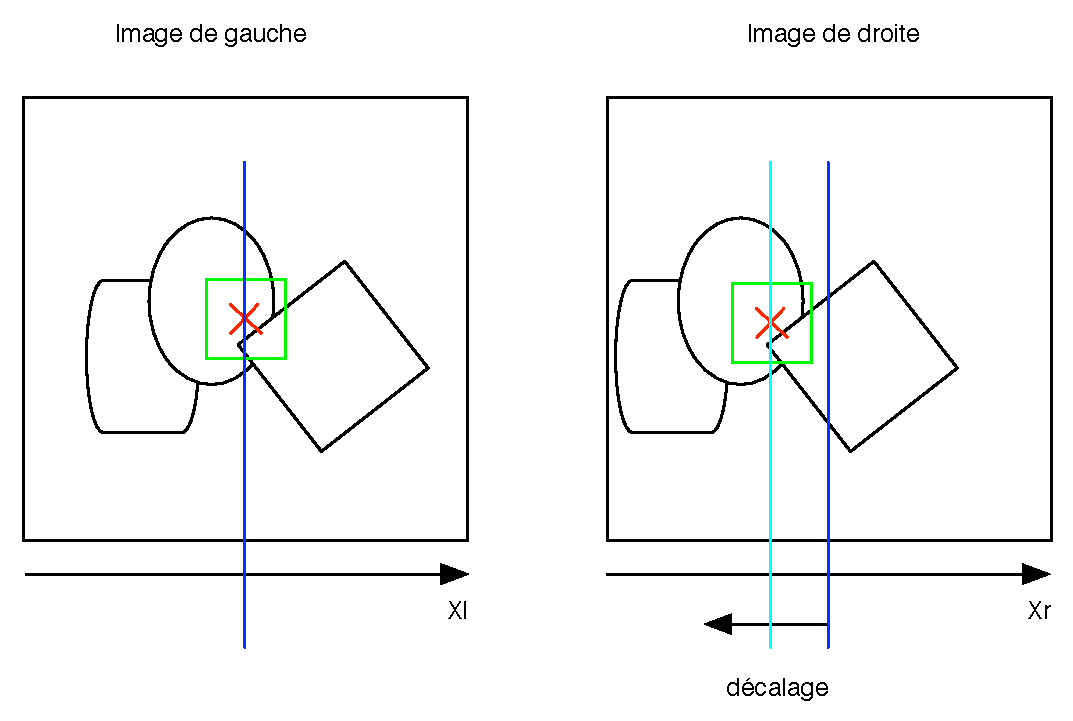
\includegraphics[width=8cm]{images/calcule_SSD}
\end{center}
	\caption{Sch\'ema du calcul de la minimisation de la dissimilarit\'e}
	\label{calcule_SSD}
\end{figure}

La fonction de dissimilarit\'e utilis\'ee sera la somme des diff\'erences au carr\'e (SSD\footnote{Sum of Squared Differences}). \\

Dans le TP on effectue cette op\'eration de calcule du SSD sur toute l'image dans la fonction \emph{iviLeftDisparityMap} avec l'image de gauche comme r\'ef\'erence et \emph{iviRightDisparityMap} avec l'image de droite comme r\'ef\'erence. \\

On va calculer pour chaque d\'ecalage le SSD que l'on va stocker dans \emph{mSSD} et on ne gardera que les valeurs pour lesquels le SSD est le minimum que l'on stockera dans \emph{mMinSSD}. On remarque aussi que dans la fonction \emph{iviLeftDisparityMap}  les pointeurs permettant d'acc\'eder aux pixels des images subissent un d\'ecalage \'egale \`a la moiti\'e de la taille du voisinage. Ceci permettant de ne pas faire de d\'epassement de tableau lors du calcule du SSD. \\

Afin d'avoir la carte des disparit\'es, pour chaque d\'ecalage on calcule le SSD avec la m\'ethode \emph{iviComputeLeftSSDCost} et on comparera les valeurs obtenu avec les autre d\'ecalages afin de r\'ecup\'erer les co\^uts (en d\'ecalage) minimum. \\

Apr\`es calcule on obtient la Fig.\ref{disparite_img_g}. \\

\begin{figure}[ht]
\begin{center}
	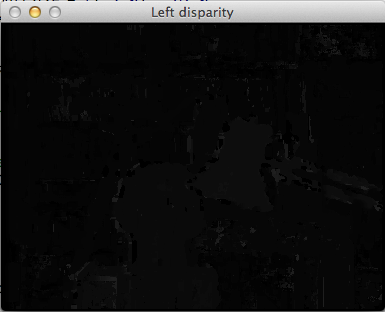
\includegraphics[width=8cm]{images/disparite_img_g.png}
\end{center}
	\caption{Carte des disparit\'es avec l'image de gauche comme r\'ef\'erence}
	\label{disparite_img_g}
\end{figure}

\newpage

Cette image est rendu visible via les deux fonctions  \emph{minMaxLoc} et \emph{normalize}. La fonction \emph{minMaxLoc} permet de r\'ecup\'erer la valeur minimum (\emph{min}) et la valeur maximum (\emph{max}) de l'image. Ensuite on effectue une normalisation sur ces deux valeurs \emph{min} et \emph{max} c'est a dire une \'egalisation de l'histogramme (\emph{cf.}~Fig.\ref{histo}).

\begin{figure}[ht]
\begin{center}
	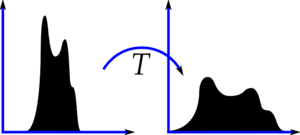
\includegraphics[width=8cm]{images/histo.png}
\end{center}
	\caption{Sch\'ema de l'\'egalisation d'un histogramme (source : \url{http://en.wikipedia.org/wiki/Histogram_equalization})}
	\label{histo}
\end{figure}


\section{V\'erification gauche-droite}

La prochaine \'etape consiste \`a faire une carte de disparit\'e qui est un combin\'e des deux cartes (gauche et droite). Dans cette carte on ne va garder que les disparit\'es de la carte gauche (ayant l'image gauche comme r\'ef\'erence) qui poss\`ede un homologue dans la carte de disparit\'e droite. \\

Pour le moment on a que la carte de disparit\'e avec l'image gauche comme r\'ef\'erence. On va maintenant calculer la carte de disparit\'e pour l'image droite en utilisant la fonction \emph{iviRightDisparityMap}. La Fig.\ref{disparite_img_d} est le r\'esultat de cette fonction.

\begin{figure}[ht]
\begin{center}
	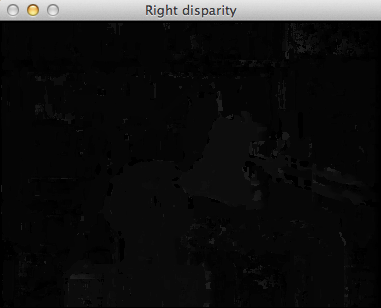
\includegraphics[width=8cm]{images/disparite_img_d.png}
\end{center}
	\caption{Carte des disparit\'es avec l'image de droite comme r\'ef\'erence}
	\label{disparite_img_d}
\end{figure}

\newpage

Ensuite avec ces deux cartes on va rechercher les disparit\'es homologues. Pour ce faire on va compl\'eter la fonction \emph{iviLeftRightConsistency} qui rempli deux matrices \emph{mValidityMask} et  \emph{mDisparity}.

 \emph{mValidityMask} correspond \`a un masque de validit\'e remplit de la fa\c con suivante : si pour un pixel la disparit\'e \`a bien \'et\'e calcul\'e alors on met 0 sinon on met 255. De ce fait les pixels marqu\'e comme incorrecte sont bien visible (\emph{cf.}~Fig.\ref{masque}).

\begin{figure}[ht]
\begin{center}
	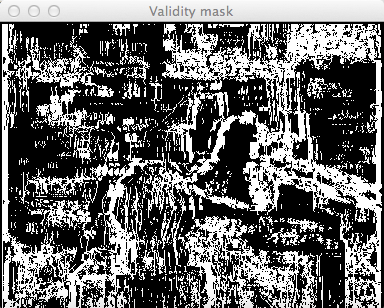
\includegraphics[width=8cm]{images/masque.png}
\end{center}
	\caption{Masque de validit\'e}
	\label{masque}
\end{figure}


Enfin gr\^ace \`a ce masque on peut r\'ecup\'erer les disparit\'es correcte, il suffit de ne prendre que les disparit\'es \`a la position ou le masque \`a comme valeur 0 (\emph{cf.}~Fig.\ref{disparite}).

\begin{figure}[ht]
\begin{center}
	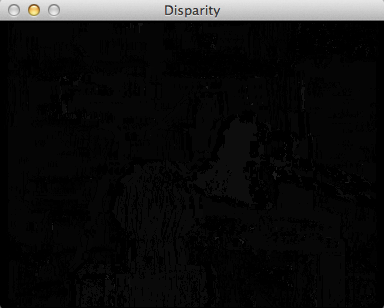
\includegraphics[width=8cm]{images/disparite.png}
\end{center}
	\caption{Carte des disparit\'es coh\'erente}
	\label{disparite}
\end{figure}


\section{Calcul efficace du SSD}

c'est 4.

\section*{Conclusion}

Cette m\'ethode de st\'er\'eovision est plus pr\'ecise que la pr\'ec\'edente car elle se base sur tout les pixels de l'image ainsi que la photom\'etrie des deux images. Mais elle s'ex\'ecute plus lentement que la pr\'ec\'edente et elle poss\`ede des contraintes li\'e \`a la photom\'etrie de chaque image.

\end{document}